\documentclass[graphic, aspectratio=169]{beamer}

\usepackage{listings}
\usepackage{graphicx}
\usepackage{caption}
\usepackage{subcaption}
\usepackage{hyperref}
\usepackage{tabularx}
\usepackage{parcolumns}
\usepackage{fontawesome}

\usepackage{color}
\definecolor{lightgray}{rgb}{0.95, 0.95, 0.95}
\definecolor{darkgray}{rgb}{0.4, 0.4, 0.4}
%\definecolor{purple}{rgb}{0.65, 0.12, 0.82}
\definecolor{editorGray}{rgb}{0.95, 0.95, 0.95}
\definecolor{editorOcher}{rgb}{1, 0.30, 0} % #FF7F00 -> rgb(239, 169, 0)
\definecolor{editorGreen}{rgb}{0, 0.5, 0} % #007C00 -> rgb(0, 124, 0)
\definecolor{orange}{rgb}{1,0.45,0.13}		
\definecolor{olive}{rgb}{0.17,0.59,0.20}
\definecolor{brown}{rgb}{0.69,0.31,0.31}
\definecolor{purple}{rgb}{0.38,0.18,0.81}
\definecolor{lightblue}{rgb}{0.1,0.57,0.7}
\definecolor{lightred}{rgb}{1,0.4,0.5}
\usepackage{upquote}
\usepackage{listings}
% CSS
\lstdefinelanguage{CSS}{
  keywords={color,background-image:,margin,padding,font,weight,display,position,top,left,right,bottom,list,style,border,size,white,space,min,width, transition:, transform:, transition-property, transition-duration, transition-timing-function},	
  sensitive=true,
  morecomment=[l]{//},
  morecomment=[s]{/*}{*/},
  morestring=[b]',
  morestring=[b]",
  alsoletter={:},
  alsodigit={-}
}

% JavaScript
\lstdefinelanguage{JavaScript}{
  morekeywords={typeof, new, true, false, catch, function, return, null, catch, switch, var, if, in, while, do, else, case, break},
  morecomment=[s]{/*}{*/},
  morecomment=[l]//,
  morestring=[b]",
  morestring=[b]'
}

\lstdefinelanguage{HTML5}{
  language=html,
  sensitive=true,	
  alsoletter={<>=-},	
  morecomment=[s]{<!-}{-->},
  tag=[s],
  otherkeywords={
  % General
  >,
  % Standard tags
	<!DOCTYPE,
  </html, <html, <head, <title, </title, <style, </style, <link, </head, <meta, />,
	% body
	</body, <body,
	% Divs
	</div, <div, </div>, 
	% Paragraphs
	</p, <p, </p>,
	% scripts
	</script, <script,
  % More tags...
  <canvas, /canvas>, <svg, <rect, <animateTransform, </rect>, </svg>, <video, <source, <iframe, </iframe>, </video>, <image, </image>, <header, </header, <article, </article
  },
  ndkeywords={
  % General
  =,
  % HTML attributes
  charset=, src=, id=, width=, height=, style=, type=, rel=, href=,
  % SVG attributes
  fill=, attributeName=, begin=, dur=, from=, to=, poster=, controls=, x=, y=, repeatCount=, xlink:href=,
  % properties
  margin:, padding:, background-image:, border:, top:, left:, position:, width:, height:, margin-top:, margin-bottom:, font-size:, line-height:,
	% CSS3 properties
  transform:, -moz-transform:, -webkit-transform:,
  animation:, -webkit-animation:,
  transition:,  transition-duration:, transition-property:, transition-timing-function:,
  }
}

\lstdefinestyle{htmlcssjs} {%
  % General design
%  backgroundcolor=\color{editorGray},
  basicstyle={\footnotesize\ttfamily},   
  frame=b,
  % Code design
  identifierstyle=\color{black},
  keywordstyle=\color{blue}\bfseries,
  ndkeywordstyle=\color{editorGreen}\bfseries,
  stringstyle=\color{editorOcher}\ttfamily,
  commentstyle=\color{brown}\ttfamily,
  % Code
  language=HTML5,
  alsolanguage=JavaScript,
  alsodigit={.:;},	
  tabsize=2,
  showtabs=false,
  showspaces=false,
  showstringspaces=false,
  extendedchars=true,
  breaklines=true,
  % German umlauts
  literate=%
  {Ö}{{\"O}}1
  {Ä}{{\"A}}1
  {Ü}{{\"U}}1
  {ß}{{\ss}}1
  {ü}{{\"u}}1
  {ä}{{\"a}}1
  {ö}{{\"o}}1
}

\setbeamertemplate{frametitle}[default][center]
\setbeamertemplate{navigation symbols}{}%remove navigation symbols
\setbeamertemplate{background}
{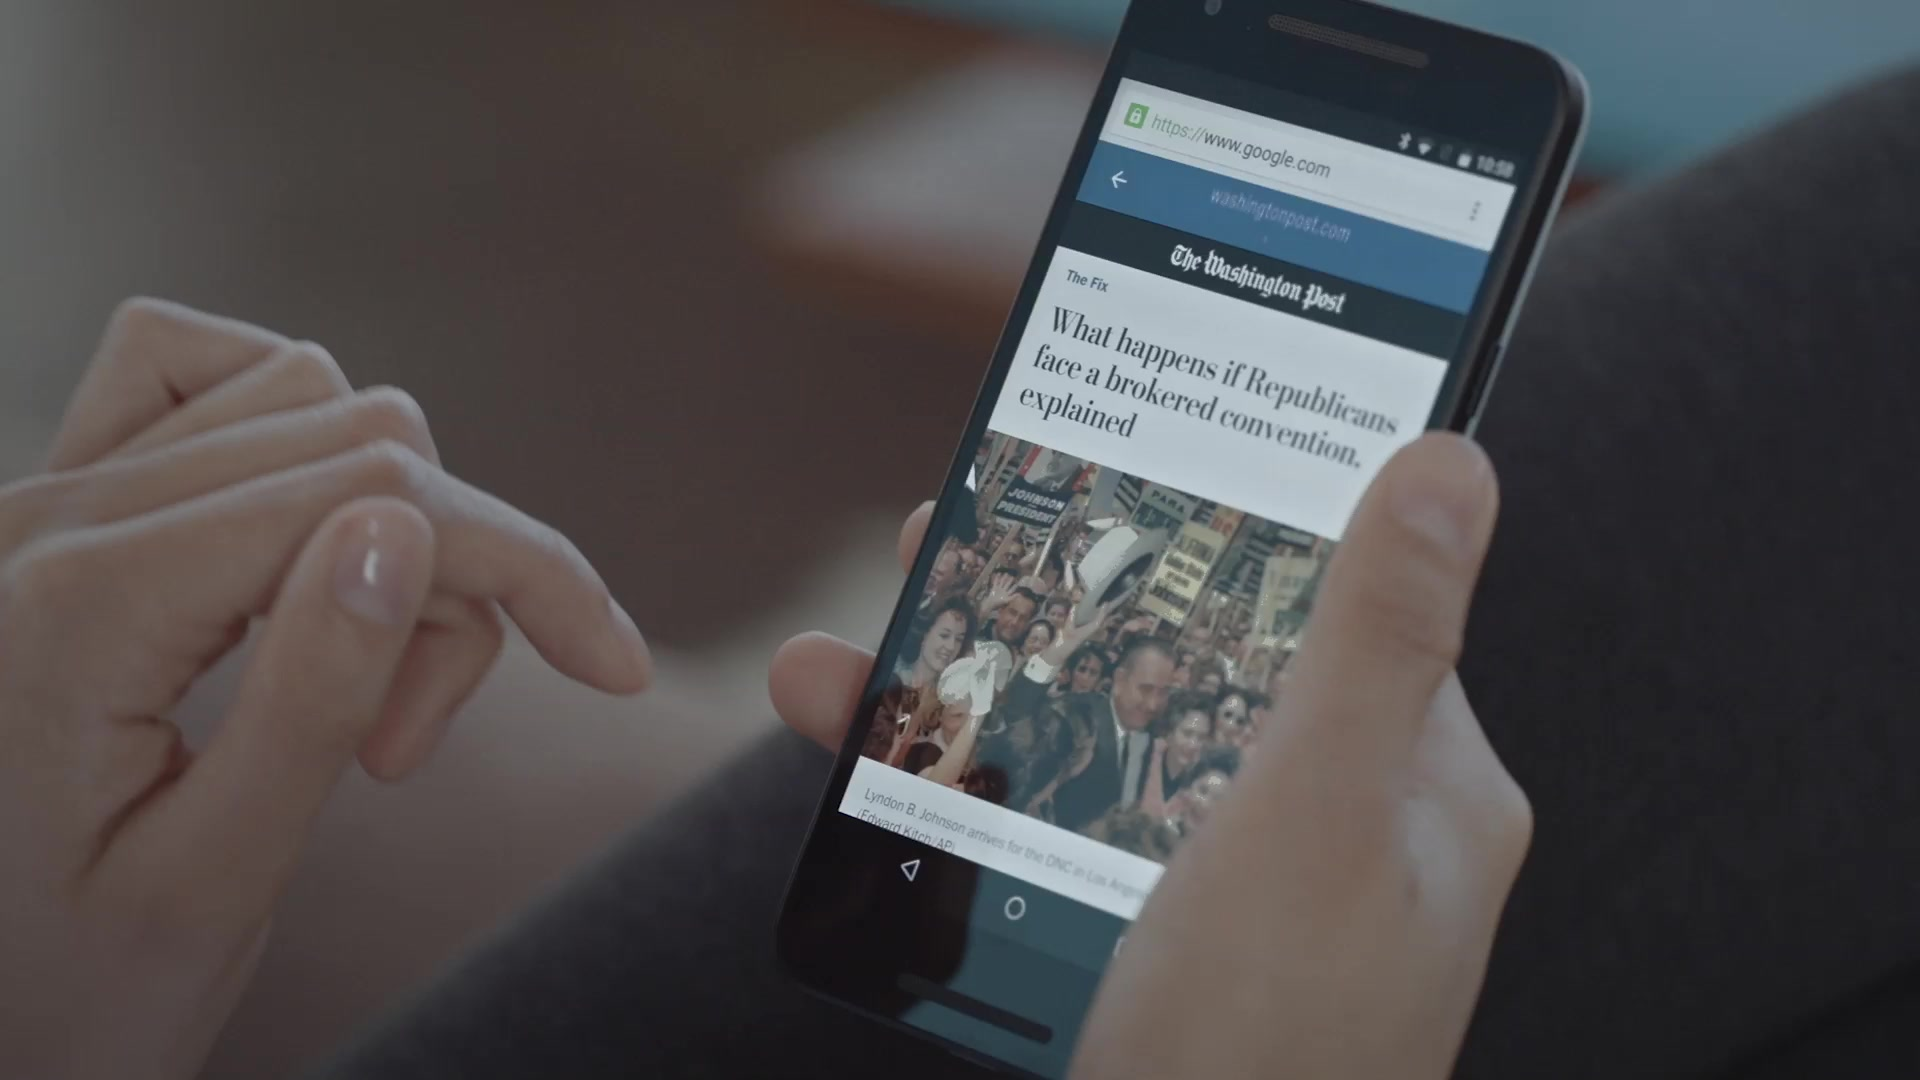
\includegraphics[width=\paperwidth,height=\paperheight,keepaspectratio=true]{images/background.jpg}}

\begin{document}

\begin{frame}
\begin{picture}(300,200)
\put(30,80){
\includegraphics[scale=.1]{images/logo-AMP}}
\put(10,60){
    \textcolor{white}{
        \begin{minipage}[t]{0.4\linewidth}
            {AMP - Accelerated Mobile Pages}
        \end{minipage}
    }
}
\end{picture}
\end{frame}

\setbeamertemplate{background}
{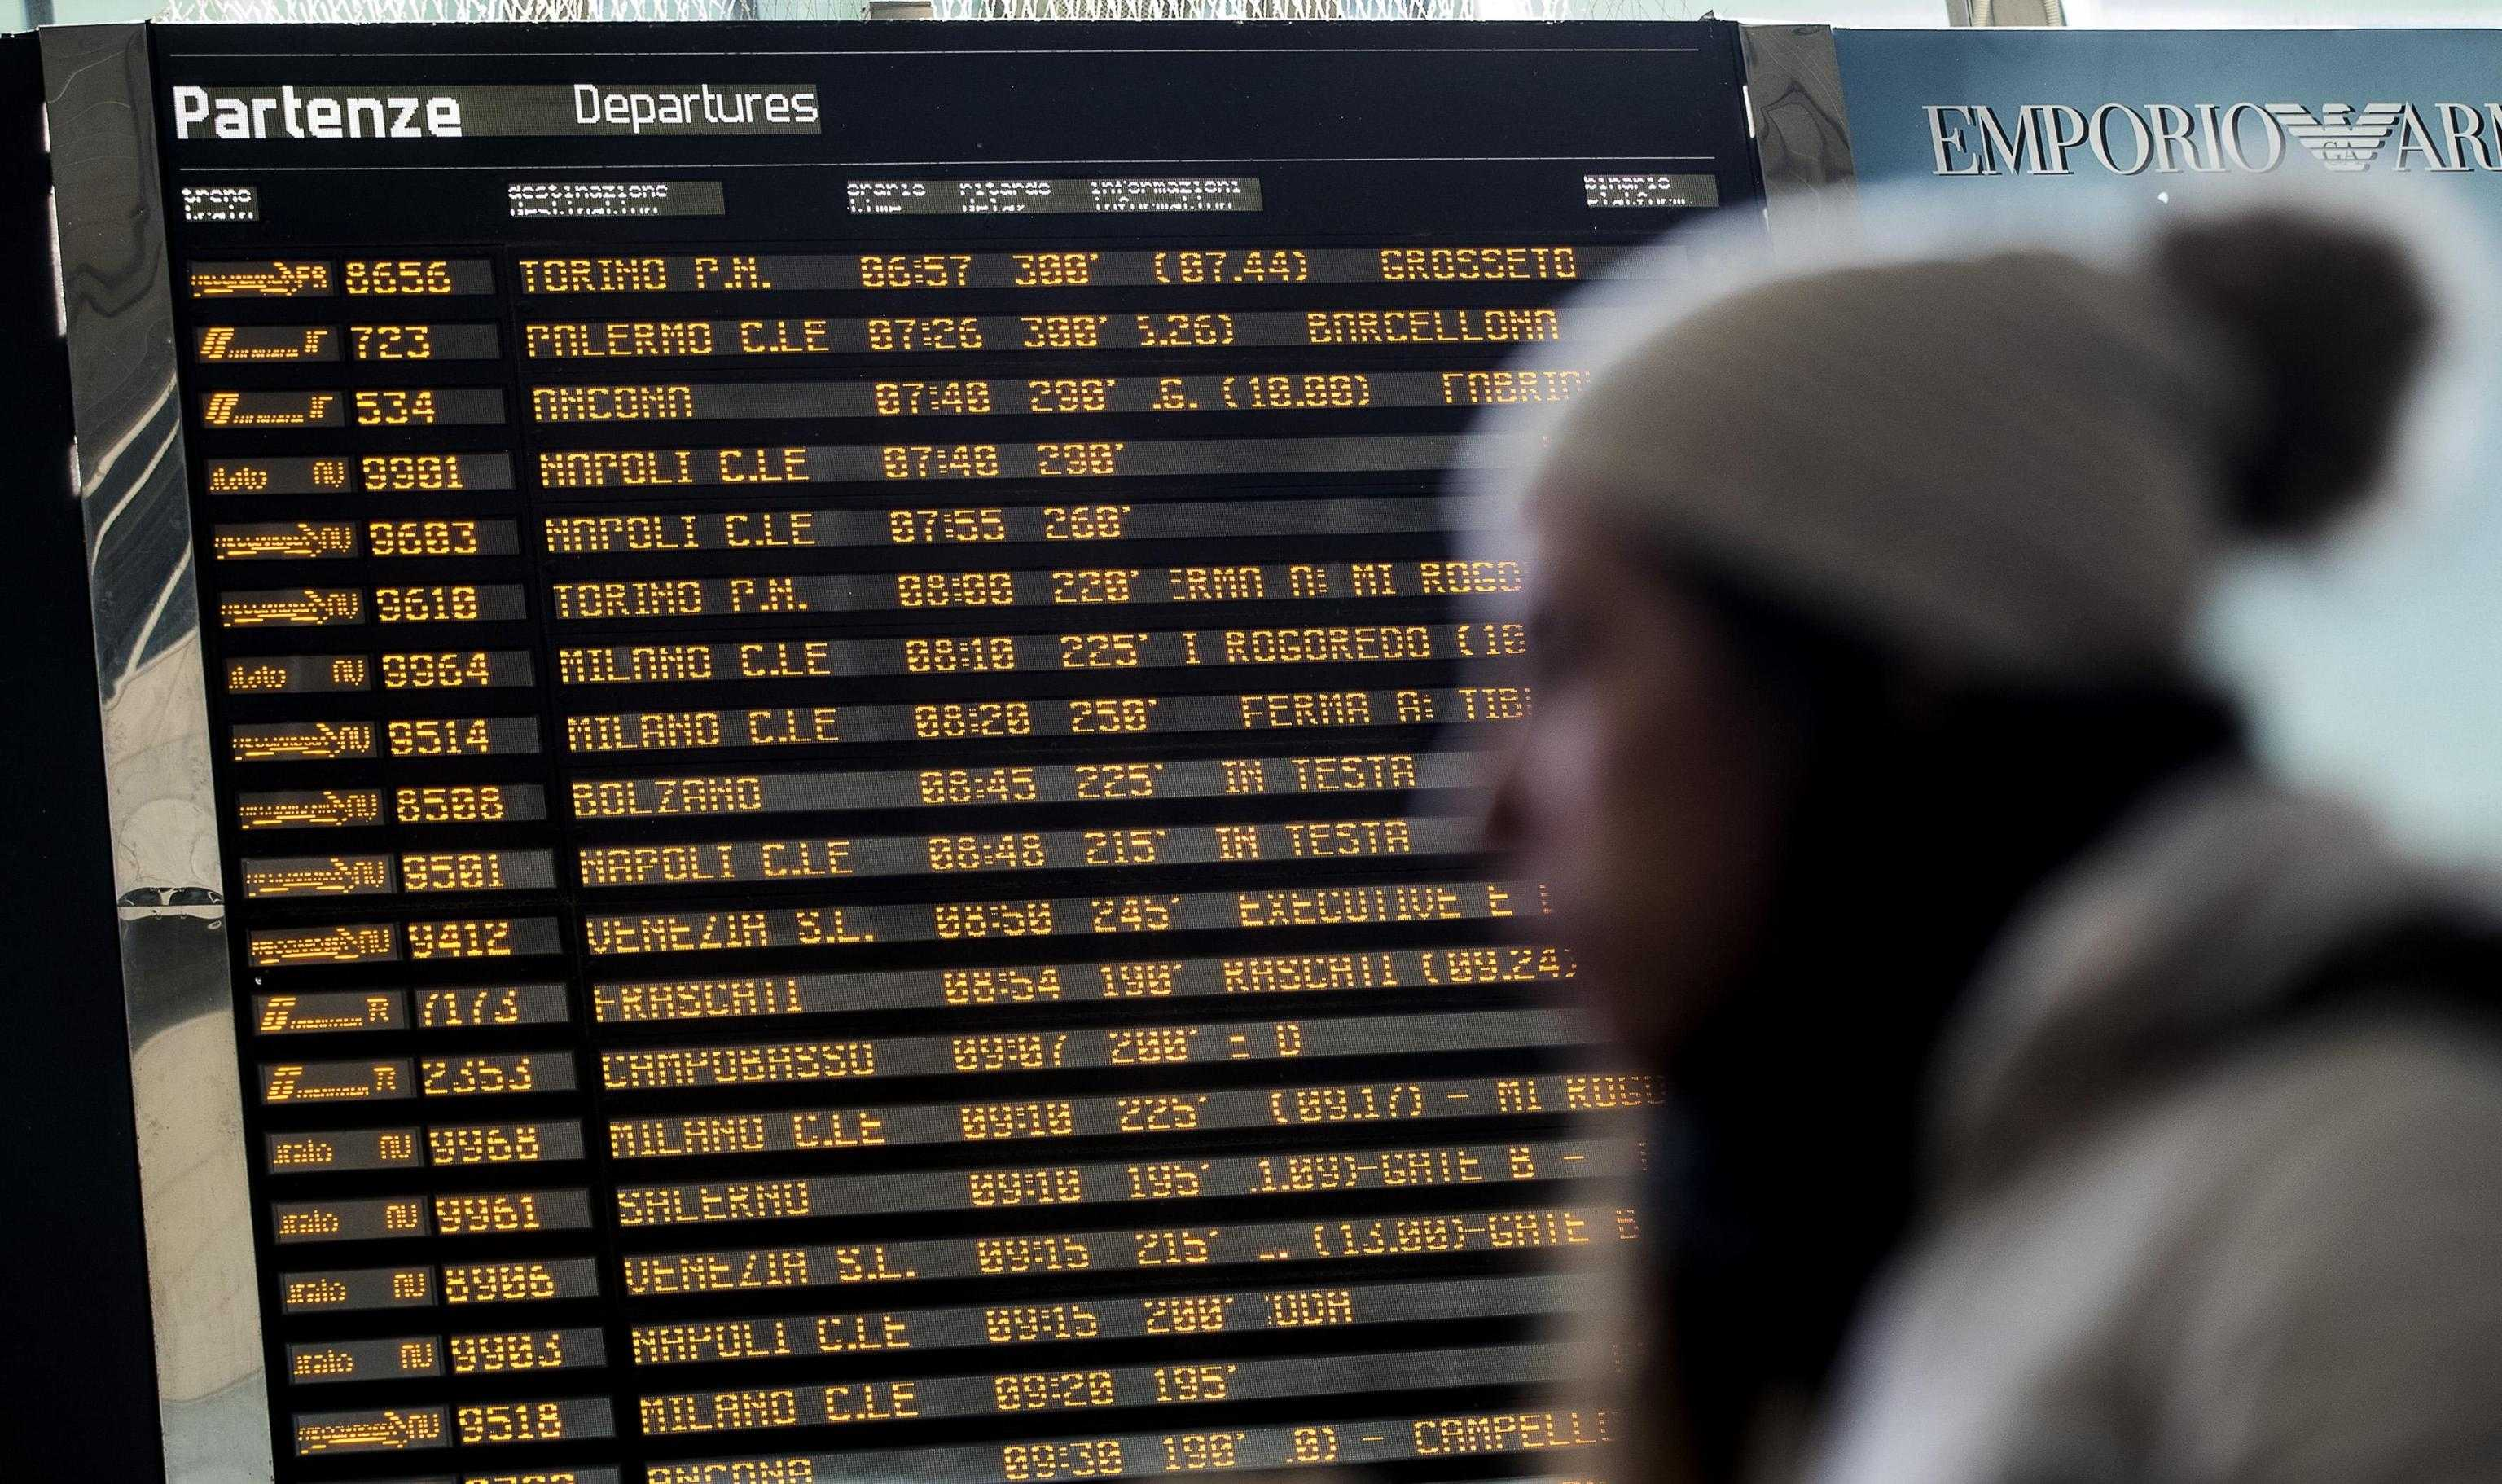
\includegraphics[width=\paperwidth,height=\paperheight]{slides/images/trenitalia_late.jpg}}
\begin{frame}
\end{frame}

\setbeamertemplate{background}
{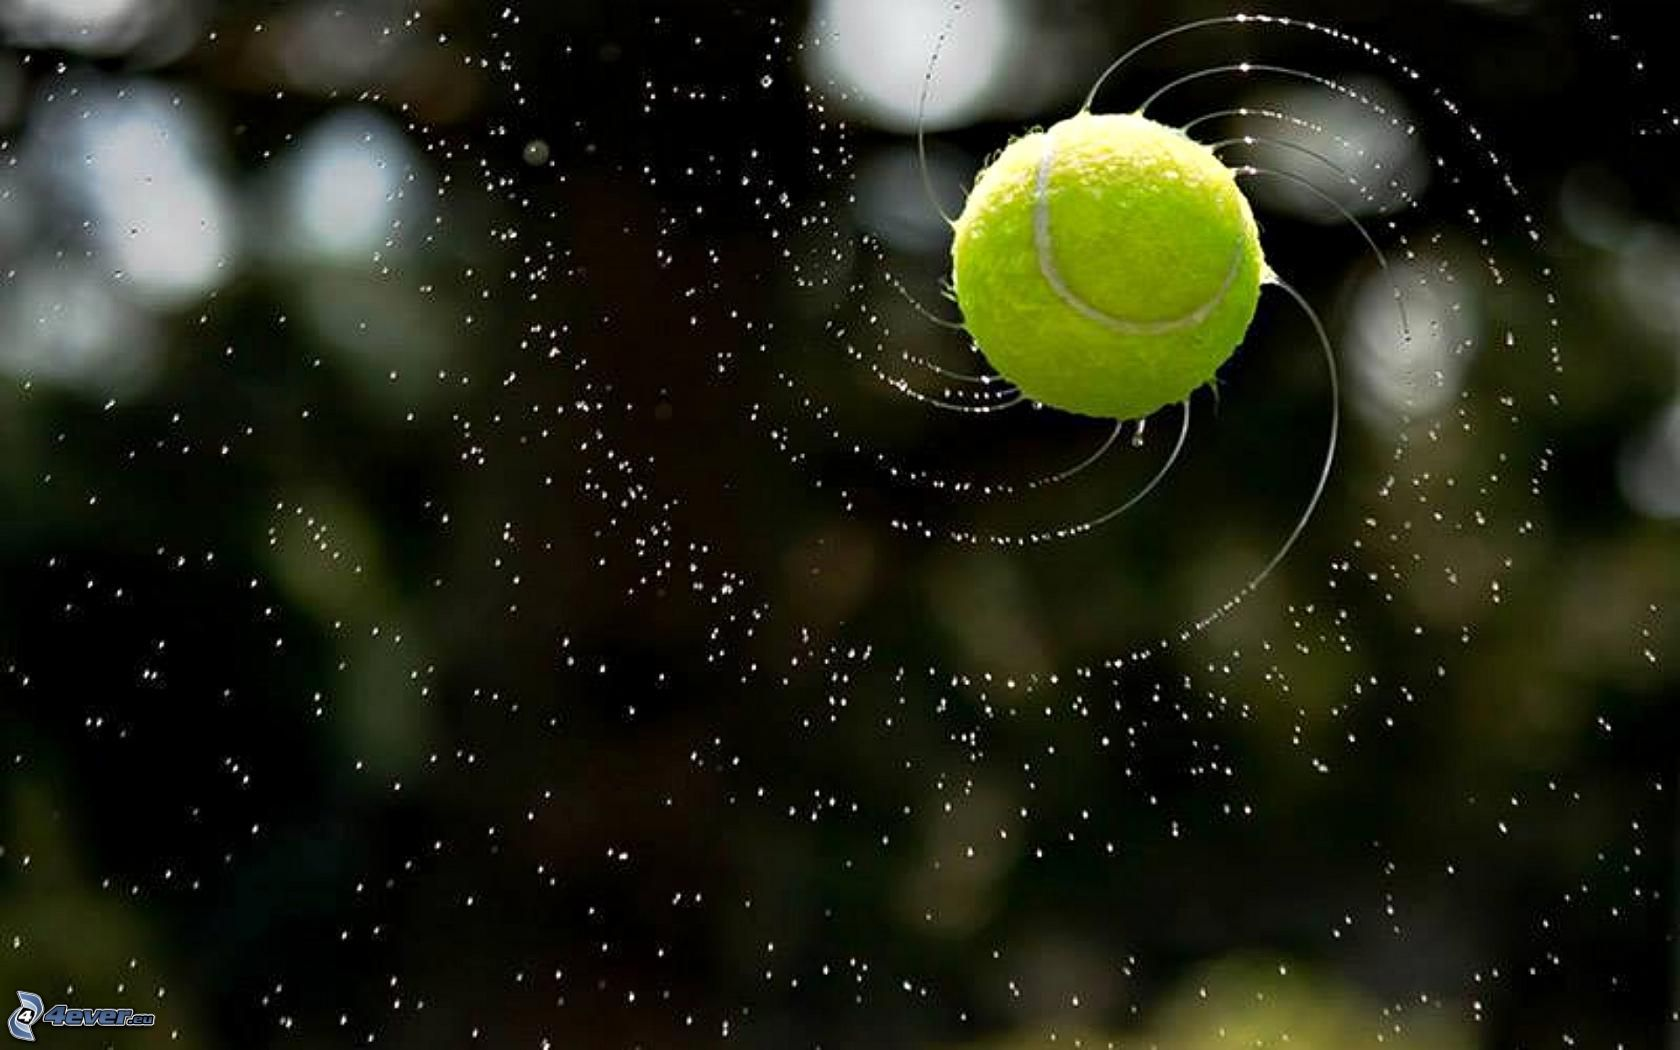
\includegraphics[width=\paperwidth,height=\paperheight]{slides/images/tennis-ball.jpg}}
\begin{frame}
\end{frame}

\setbeamertemplate{background}{} % Imposto il background bianco 

\begin{frame}
    % AMP is a way to build web pages for static content that render fast. AMP in action consists of three different parts:
    % html-amp, AMP js, Google AMP Cache
    \begin{figure}[h!]
    \centering
    
\includegraphics[scale=0.1]{images/logo-AMP.png}
    \label{fig:AMP logo}
    \end{figure}
    \begin{center}
    AMP HTML   -   AMP JS  -  Google AMP Cache
    \end{center}
\end{frame}

\setbeamertemplate{background}
{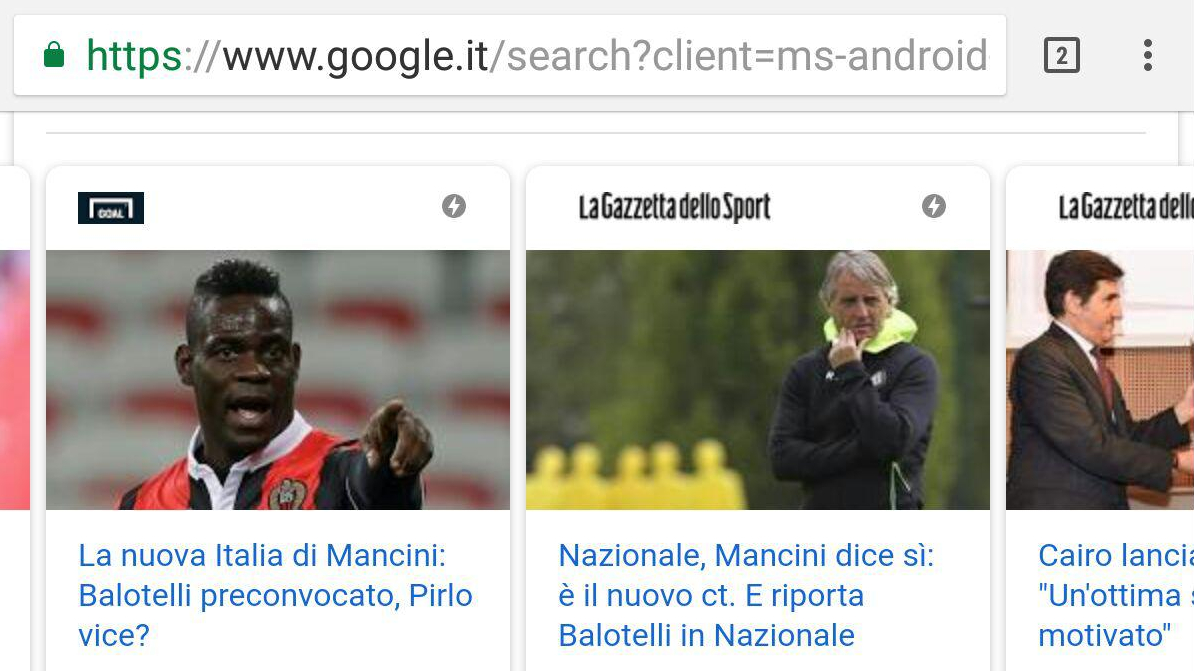
\includegraphics[width=\paperwidth,height=\paperheight]{slides/images/amp_nazionale_italiana.jpg}}
\begin{frame}
\end{frame}

\setbeamertemplate{background}{}
\begin{frame}    
    \begin{figure}[h!]
    \centering
    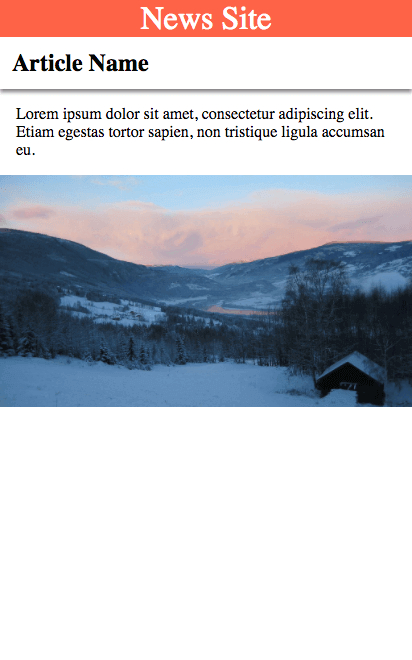
\includegraphics[scale=0.5]{slides/images/article-screenshot.png}
    \label{fig:AMP logo}
    \end{figure}
\end{frame}
    
\begin{frame}    
    \lstinputlisting[style=htmlcssjs, frame=single]{code/html/article.html}
\end{frame}

\begin{frame}
\noindent\begin{minipage}{.40\textwidth}
    \lstinputlisting[style=htmlcssjs, frame=single]{code/html/article-html-tag.html}
\end{minipage}\hfill
\begin{minipage}{.55\textwidth}
    \lstinputlisting[style=htmlcssjs, frame=single]{code/amp/article-html-tag.html}
    % <script async ... >Includes and loads the AMP JS library
    % The AMP runtime is a piece of JavaScript that runs inside every AMP document. It provides implementations for AMP custom elements, manages resource loading and prioritization and optionally includes a runtime validator for AMP HTML for use during development.

%The AMP runtime is loaded via the mandatory <script src="https://cdn.ampproject.org/v0.js"></script> tag in the AMP document <head>.
\end{minipage}
\end{frame}

\begin{frame}
\noindent\begin{minipage}{.40\textwidth}
    \lstinputlisting[style=htmlcssjs, frame=single]{code/html/article-link-rel.html}
\end{minipage}\hfill
\begin{minipage}{.55\textwidth}
    \lstinputlisting[style=htmlcssjs, frame=single]{code/amp/article-link-rel.html}
\end{minipage}
\end{frame}

\begin{frame}
\noindent\begin{minipage}{.40\textwidth}
    \lstinputlisting[style=htmlcssjs, frame=single]{code/html/article-viewport.html}
\end{minipage}\hfill
\begin{minipage}{.55\textwidth}
    \lstinputlisting[style=htmlcssjs, frame=single]{code/amp/article-viewport.html}
\end{minipage}
\end{frame}

\begin{frame}
\noindent\begin{minipage}{.40\textwidth}
    \lstinputlisting[style=htmlcssjs, frame=single]{code/html/article-css.html}
\end{minipage}\hfill
\begin{minipage}{.55\textwidth}
    \lstinputlisting[style=htmlcssjs, frame=single]{code/amp/article-css.html}
\end{minipage}
\end{frame}

\begin{frame}    
    \lstinputlisting[style=htmlcssjs, frame=single]{code/html/article-js.html}
\end{frame}

\begin{frame}
\noindent\begin{minipage}{.40\textwidth}
    \lstinputlisting[style=htmlcssjs, frame=single]{code/html/article-image.html}
\end{minipage}\hfill
\begin{minipage}{.55\textwidth}
    \lstinputlisting[style=htmlcssjs, frame=single]{code/amp/article-image.html}
\end{minipage}
\end{frame}

\setbeamertemplate{background}
{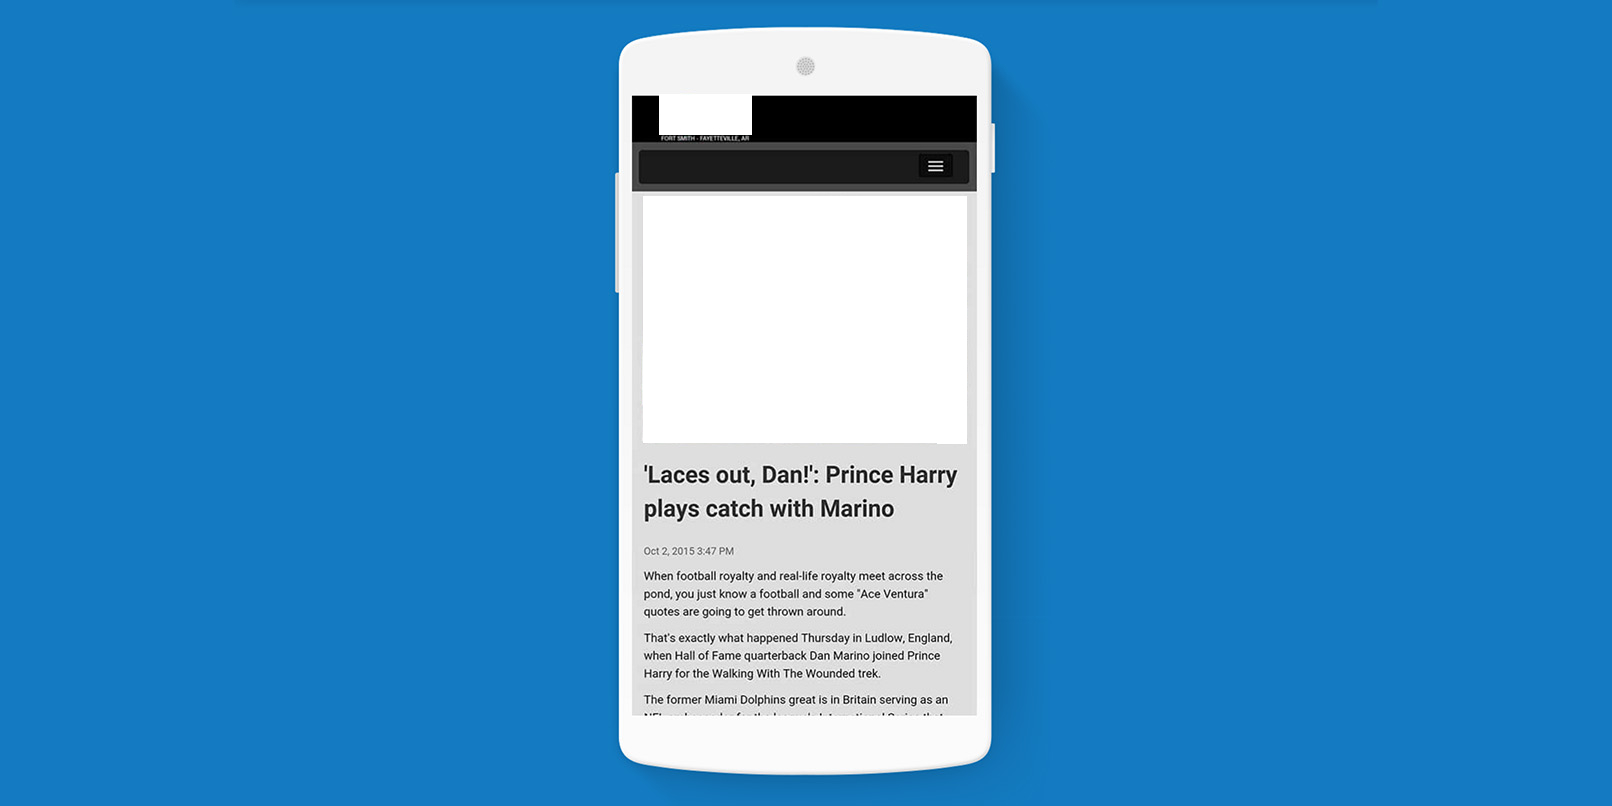
\includegraphics[width=\paperwidth,height=\paperheight]{slides/images/amp_example_without_images.jpg}}
\begin{frame}
\end{frame}

\setbeamertemplate{background}
{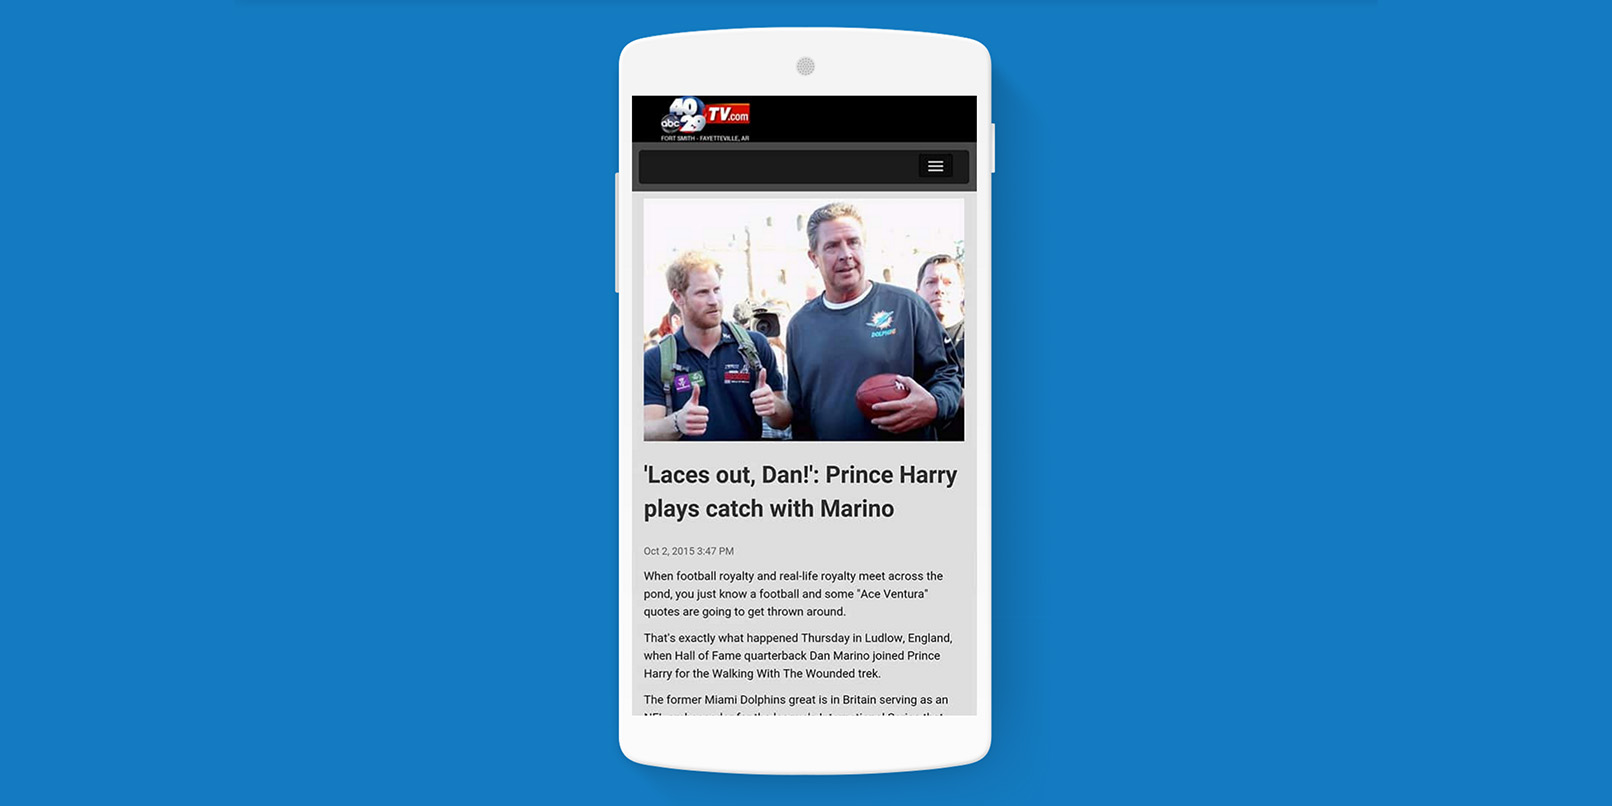
\includegraphics[width=\paperwidth,height=\paperheight]{images/amp_example.jpg}}
\begin{frame}
\end{frame}

\setbeamertemplate{background}{}

\begin{frame}
\noindent\begin{minipage}{.45\textwidth}
    \lstinputlisting[style=htmlcssjs, frame=single]{code/amp/article.amp-1.html}
\end{minipage}\hfill
\begin{minipage}{.45\textwidth}
    \lstinputlisting[style=htmlcssjs, frame=single]{code/amp/article.amp-2.html}
\end{minipage}
\end{frame}

\setbeamertemplate{background}
{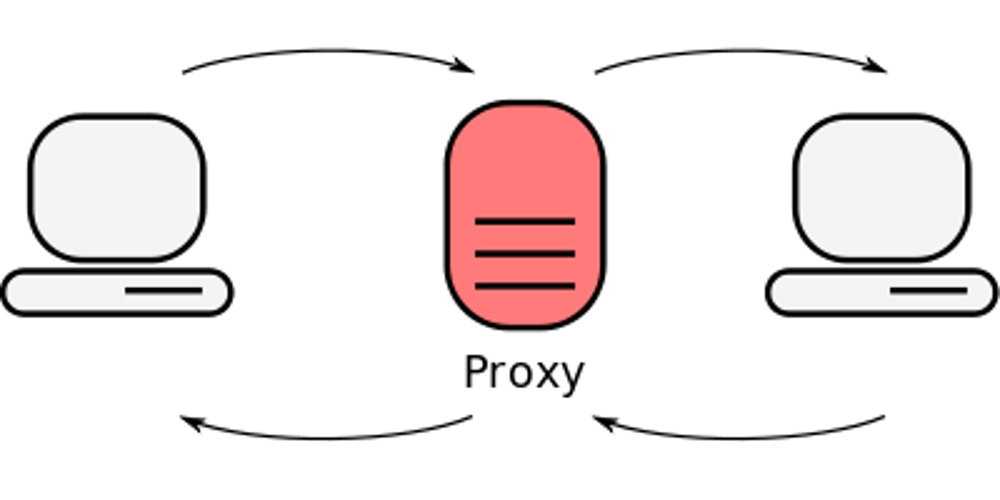
\includegraphics[width=\paperwidth,height=\paperheight]{images/proxy.png}}
\begin{frame}{AMP Cache}
\end{frame}

\setbeamertemplate{background}
{\href{https://search.google.com/test/amp?view=search-preview&id=srqIZ15g1kFY89ACklbuMA}{
\includegraphics[width=\paperwidth]{slides/images/repubblica_phone.png}}}
\begin{frame}
\end{frame}

\setbeamertemplate{background}
{
\includegraphics[width=\paperwidth,height=\paperheight]{slides/images/dislike.jpg}}
\begin{frame}
\end{frame}

\setbeamertemplate{background}
{
\includegraphics[width=\paperwidth]{slides/images/repubblica_phone.png}}
\begin{frame}
\end{frame}

\setbeamertemplate{background}
{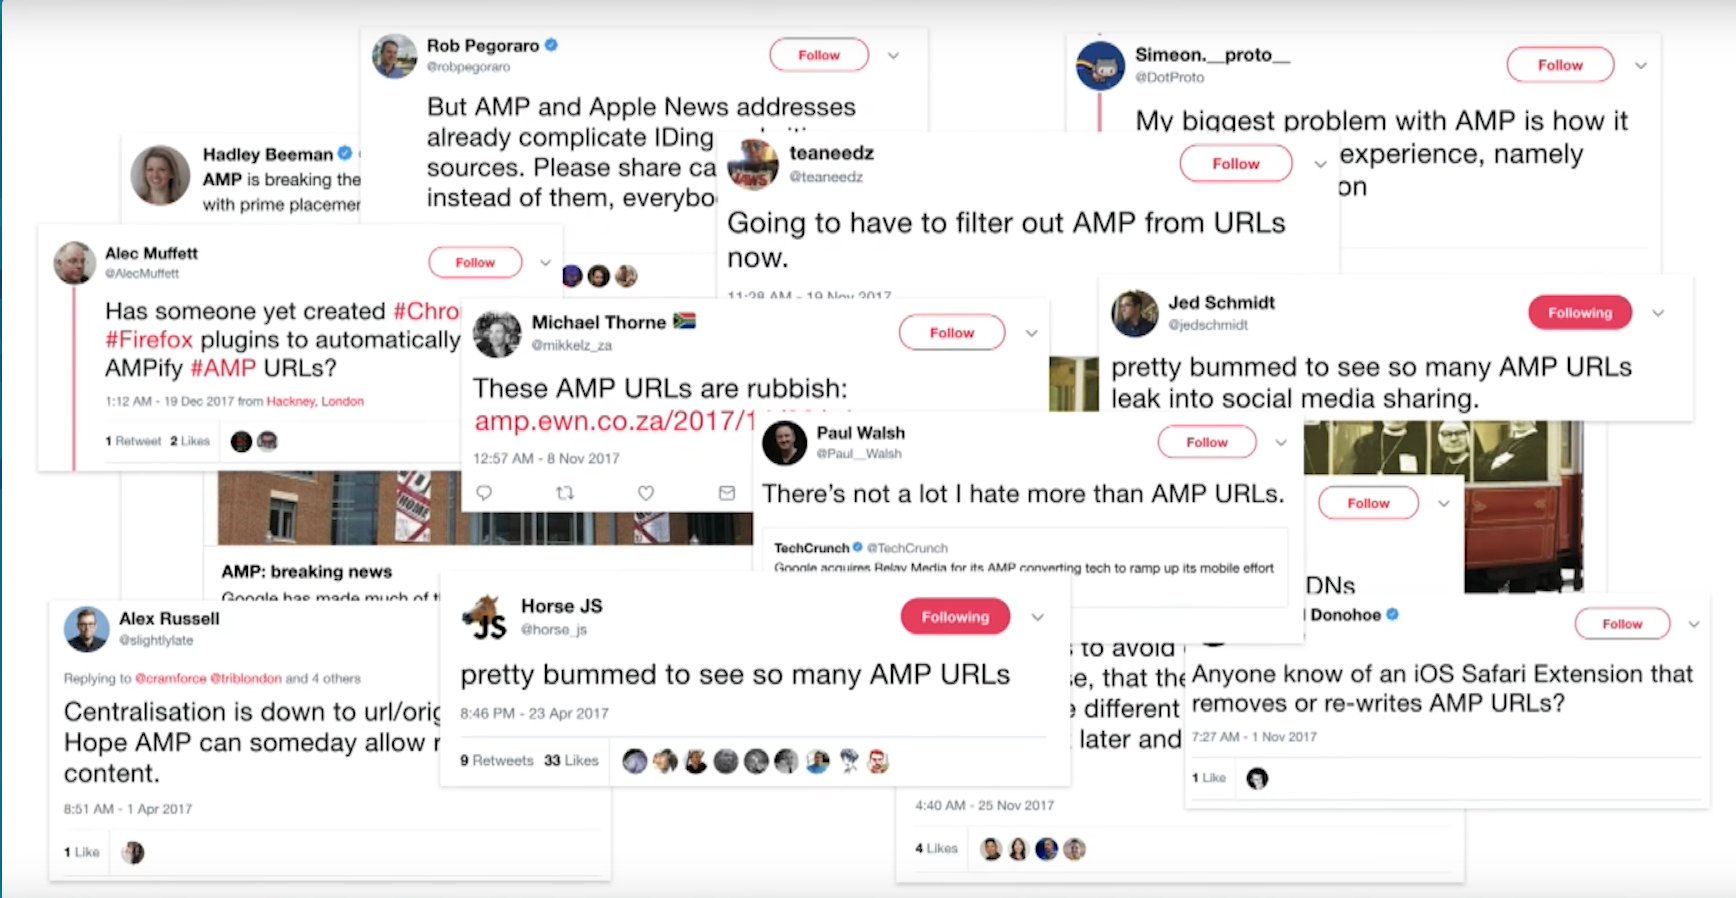
\includegraphics[width=\paperwidth,height=\paperheight]{slides/images/against_amp.png}}
\begin{frame}
\end{frame}

\setbeamertemplate{background}
{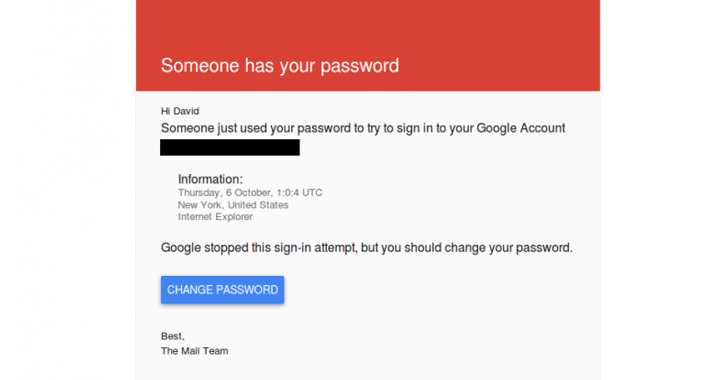
\includegraphics[width=\paperwidth,height=\paperheight]{slides/images/gmail-phishing.png}}
\begin{frame}
\end{frame}

\setbeamertemplate{background}
{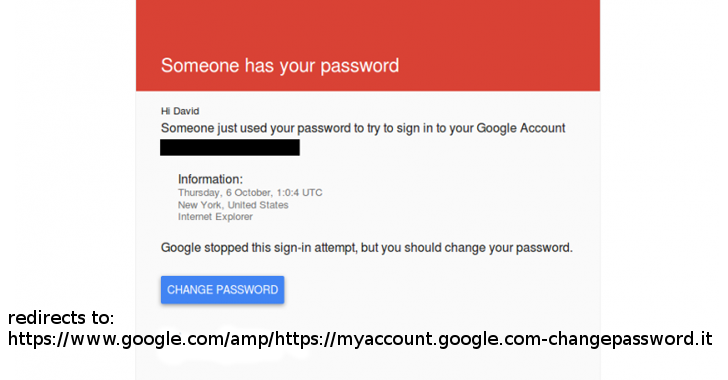
\includegraphics[width=\paperwidth,height=\paperheight]{slides/images/gmail-phishing-with-redirect.png}}
\begin{frame}
\end{frame}

\setbeamertemplate{background}{}
\begin{frame}
\begin{center}
\begin{tabular}{>{\centering\arraybackslash}p{4cm}}

\includegraphics[height=1cm]{images/twitter_logo.png} \textbf{\href{https://twitter.com/enrico_salvucci}{ @enrico\_salvucci}} \\

\includegraphics[height=1cm]{images/github_logo.png} \textbf{\href{https://github.com/esalvucci}{https://github.com/esalvucci}} \\
\end{tabular}

\bigskip
\begin{footnotesize}
Slides written in \LaTeX\ and released under \\ \textbf{\href{http://creativecommons.org/licenses/by-sa/4.0/}{Creative Commons - Attributions, Share-alike 4.0}} license.\\

\medskip

\includegraphics[height=0.8cm]{images/cc.png}

\medskip
Sources on \textbf{\url{https://github.com/esalvucci/AMP-talk}}\\
A readable version of this talk is available at \url{ https://github.com/esalvucci/AMP-talk/raw/master/readable/readable.pdf} 
\end{footnotesize}
\end{center}
\end{frame}
% https://github.com/esalvucci/AMP-talk/raw/master/readable/readable.pdf
\end{document}

